\documentclass[8pt]{beamer}\usepackage[]{graphicx}\usepackage[]{color}

%\setbeamercovered{transparent}

\usefonttheme{professionalfonts} % using non standard fonts for beamer
\usefonttheme{serif} % default family is serif
\usepackage{fontspec}
\setmainfont{Liberation Serif}

\input{_headers}


\def\argmax#1{\mathrm{argmax}_{#1}\,}
\def\argmin#1{\mathrm{argmin}_{#1}\,}
\def\cov#1#2{\mathrm{Cov}_{#1}\left( #2\right)\,}
\def\expect#1#2{\mathbb{E}_{#1}\left[ #2\right]\,}
\def\var#1#2{\mathrm{Var}_{#1}\left( #2\right)\,}
\def\cumulant#1#2{\mathcal{K}_{#1}\left( #2\right)\,}
\def\expecthat#1#2{\hat{\mathbb{E}}_{#1}\left[ #2\right]\,}
\newcommand{\fracat}[3]{\left. \frac{#1}{#2} \right|_{#3}}
\newcommand{\norm}[1]{\left\Vert#1\right\Vert}
\newcommand{\abs}[1]{\left|#1\right|}
\def\diag#1{\textrm{Diag}\left( #1\right)}
\def\ord#1{\mathcal{O}\left( #1\right)}
\def\ordp#1{\mathcal{O}_p\left( #1\right)}
\def\gauss#1{\mathcal{N}\left( #1\right)}
\def\trans{\intercal} % transpose
\def\id{I} % Identity matrix
\def\iid{\overset{iid}{\sim}}
\def\rdom#1{\mathbb{R}^{#1}}
\def\ind#1{\mathbb{I}\left(#1\right)}
\def\varemp#1{\hat{\mathrm{Var}}\left(#1\right)}
\def\eqcheck{\overset{\textrm{check}}{=}}


\def\p{\mathcal{P}}
\def\post{\p(\x \vert \y)}

\def\x{\mathbf{x}}
\def\m{\mathbf{m}}
\def\y{\mathbf{y}}
\def\xhat{\hat{\x}}
\def\s{s}
\def\S{\mathbf{s}}

\def\t{t}


\def\H{\mathbf{H}}
\def\B{\mathbf{B}}
\def\R{\mathbf{R}}
\def\Vhat{\hat{\mathbf{V}}}

\def\a{\mathbf{a}}
\def\A{\mathbf{A}}
\def\r{\mathbf{r}}



\title{Uncertainty and Model Checking for Atmospheric Inversions}
\author{Sequoia Andrade, Danika Heaney, Ron Cohen, Ryan Giordano}

\date{June 2026}

\setbeamertemplate{Collaborators}[none]
\IfFileExists{upquote.sty}{\usepackage{upquote}}{}


\begin{document}

\maketitle


\def\sectionslide#1{
\begin{frame}
   \centering
   \huge{\textbf{#1}}
\end{frame}
}

%%%%%%%%%%%%%%%%%%%%%%%%%%%%%%%%%%%%%
%%%%%%%%%%%%%%%%%%%%%%%%%%%%%%%%%%%%%
%%%%%%%%%%%%%%%%%%%%%%%%%%%%%%%%%%%%%

\begin{frame}{Model}

What we know, and what we want to know:
%
$$
\begin{aligned}
\y:{}& \textrm{Observed measurements} &\textrm{dimension } M\\
\x:{}& \textrm{Unobserved flux} &\textrm{dimension } N\\
\end{aligned}
$$

Hyperparemters and data generating process:

$$
\begin{aligned}
\H:{}& \textrm{Footprints} &\textrm{dimension } M \times N\\
\B:{}& \textrm{Prior covariance} &\textrm{dimension } N \times N\\
\R:{}& \textrm{Observation error} &\textrm{dimension } M \times M\\
\m:{}& \textrm{Prior inventory} &\textrm{dimension } N\\
\end{aligned}
$$

$$
\begin{aligned}
\y \sim{}& \gauss{\m, \B} & 
   \textrm{Actual fluxes are smooth, centered at inventory} \\
\x \vert \y \sim{}& \gauss{\H \y, \R} & 
   \textrm{The footprints transport }\y\textrm{, then observe with some error} \\
\end{aligned}
$$

\pause

Inversions estimate $\xhat = \expect{\post}{\x}$ at great expense!   

Would also like, without a ton of extra computation:
%
\begin{itemize}
\item Measurements of posterior uncertainty. (E.g., how large is $\cov{\post}{\x}$?)
\item Measurements of prior sensitivity (E.g., what if the length scale of $\B$ changed?)
\item Measurements of data influence (E.g., how much is my data, and how much my prior?)
\end{itemize}
%


\end{frame}



%%%%%%%%%%%%%%%%%%%%%%%%%%%%%%%%%%%%%
%%%%%%%%%%%%%%%%%%%%%%%%%%%%%%%%%%%%%
%%%%%%%%%%%%%%%%%%%%%%%%%%%%%%%%%%%%%

\begin{frame}{Inference}

Data generating process:
$$
\begin{aligned}
\y \sim{}& \gauss{\m, \B} & 
   \textrm{Actual fluxes are smooth, centered at inventory} \\
\x \vert \y \sim{}& \gauss{\H \y, \R} & 
   \textrm{The footprints transport }\y\textrm{, observed with some error} \\
\end{aligned}
$$

Inference: $\p(\y,\x)$ is Gaussian $\Rightarrow$ $\post$ is Gaussian.

$$
\begin{aligned}
   \p(\x \vert \y) ={}& \gauss{\xhat, \Vhat} \quad\textrm{where}\\
   \xhat ={}& \m + (\H \B)^\trans \left(
      \H \B \H^\trans + \R
    \right)^{-1} \left(\y - \m \right) \\
   \Vhat ={}& \B - (\H \B)^\trans \left(
      \H \B \H^\trans + \R
   \right)^{-1} (\H \B) \\
\end{aligned}
$$

\pause

Inversions estimate $\xhat = \expect{\post}{\x}$.  This is slow because of
%
\begin{itemize}
\item Forming $\H$ and $\B$ in memory
\item Computing $\H \B$ and $\H \B \H^\trans$
\item Inverting $\left(\H \B \H^\trans + \R\right)$
\end{itemize}
%
Sequoia has sped these up, and also saved to disk what she can.

\textbf{Assume we can re-use these computations.}  Let's get posterior
uncertainty, prior sensitivity, and data influence.


\end{frame}


%%%%%%%%%%%%%%%%%%%%%%%%%%%%%%%%%%%%%
%%%%%%%%%%%%%%%%%%%%%%%%%%%%%%%%%%%%%
%%%%%%%%%%%%%%%%%%%%%%%%%%%%%%%%%%%%%

\begin{frame}[t]{Posterior uncertainty}
$$
\begin{aligned}
   \p(\x \vert \y) ={}& \gauss{\xhat, \Vhat} 
   \textrm{ where }\Vhat \textrm{ is huge }(N \times N)\\
\end{aligned}
$$
\textbf{Problem:} Obviously we can't compute $\Vhat$, it is huge. 

\textbf{Idea:} We actually want to know is not $\x$, but
linear combinations of $\x$.

%%%%%%%%%
\only<2>{

\textbf{Example:} Want $\s$, the total emissions in hour $t$,
summed over all spatial locations.  

Let $\a$ be an $N-$vector with:
$$
\a_n = 
\begin{cases}
   1 &\textrm{If observation }n\textrm{ was at time }t\\
   0 &\textrm{otherwise}\\
\end{cases}
$$
Then
$$
\begin{aligned}
   \s ={}& \sum_{n=1}^N \a_n \x_n = \a^\trans \x  \Rightarrow \\
   \cov{\post}{\s} ={}&
      \cov{\post}{\a^\trans \x} ={}
      \a^\trans \cov{\post}{\x} \a
\end{aligned}
$$

\textbf{The covariance of the scalar $\s$ is a linear combination of
stuff we computed for $\xhat$:}

$$
\cov{\post}{\s} =
\a^\trans 
\underbrace{\B}_{\textrm{done}} 
\a - 
(\underbrace{\H \B}_{\textrm{done}} \a)^\trans 
\underbrace{\left(
      \H \B \H^\trans + \R
   \right)^{-1}}_{\textrm{done}} 
(\underbrace{\H \B}_{\textrm{done}} \a)
$$
}


%%%%%%%%%
\only<3>{

\textbf{Example:} Want $\S$, the total emissions in hours
$t=1,\ldots,24$, summed over all spatial locations.  

Let $\A$ be an $24 \times N$ matrix with:
$$
\A_{tn} = 
\begin{cases}
   1 &\textrm{If observation }n\textrm{ was at time }t\\
   0 &\textrm{otherwise}\\
\end{cases}
$$
Then
$$
\begin{aligned}
   \S ={}& \A \x  \Rightarrow \\
   \cov{\post}{\S} ={}&
      \A \cov{\post}{\x} \A^\trans
\end{aligned}
$$

\textbf{The covariance of the vector $\S$ is a linear combination of
stuff we already computed.}

}


%%%%%%%%%
\only<4>{

\textbf{Extreme example:} Want $\t^*$, the hour of the
day where the total flux is largest.

The value $\t^*$ is not a linear combination of $\x$.  But
we just showed that
$$
\p(\S \vert \y)  = \gauss{\A \xhat, \A \Vhat \A^\trans},
$$
and everything is computable.  So we can:
%
\begin{itemize}
\item Draw $\S_1,\ldots, \S_K$ from the multivariate normal
\item Compute $\t_k^* = \argmax{t} \S_{kt}$
\item Estimate $\var{\post}{\t^*} \approx \frac{1}{K} \sum_{k=1}^K (\t_k^* - \overline{\t^*})^2$
\end{itemize}
%

\textbf{The covariance of the vector $\t^*$ easily estimated from
stuff we already computed.}


}


\end{frame}   


%%%%%%%%%%%%%%%%%%%%%%%%%%%%%%%%%%%%%
%%%%%%%%%%%%%%%%%%%%%%%%%%%%%%%%%%%%%
%%%%%%%%%%%%%%%%%%%%%%%%%%%%%%%%%%%%%

\begin{frame}[c]{Variance (Tentative preliminary results!)}

\begin{center}
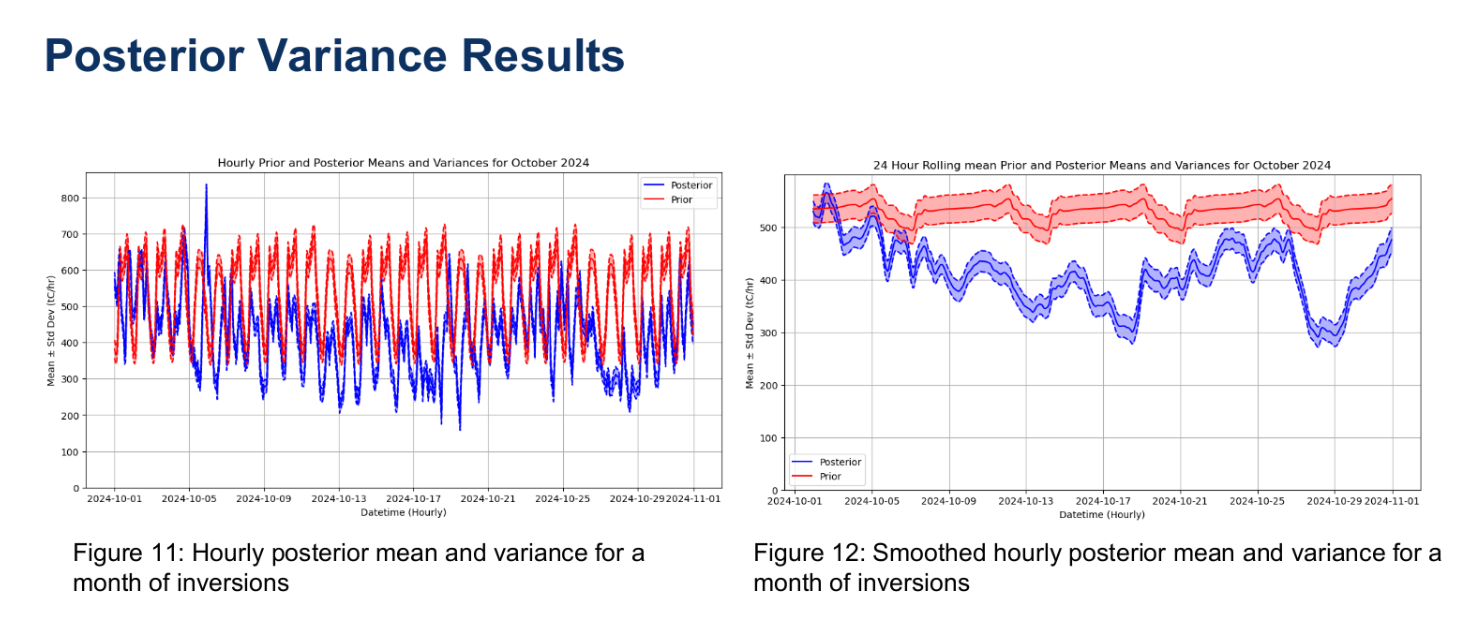
\includegraphics[width=0.8\textwidth]{static_figures/variance.png}
\end{center}

\end{frame}


%%%%%%%%%%%%%%%%%%%%%%%%%%%%%%%%%%%%%
%%%%%%%%%%%%%%%%%%%%%%%%%%%%%%%%%%%%%
%%%%%%%%%%%%%%%%%%%%%%%%%%%%%%%%%%%%%

\begin{frame}[t]{Prior sensitivity}

The prior $\B$ depends on quantities like $\rho$, an
assumed lengthscale.  So we might write
$$
\begin{aligned}
\xhat(\rho) ={}& \m + (\H \B(\rho))^\trans \left(
   \H \B(\rho) \H^\trans + \R
   \right)^{-1} \left(\y - \m \right) 
\end{aligned}
$$
\pause
\textbf{Problem:}
%
\begin{itemize}
\item Re-computing $\xhat(\rho)$ for a new lengthscale is expensive (a whole new problem).
\item There actually can be lots of hyperparameters, and you don't know which matter.
\end{itemize}
%

\pause
\textbf{Idea:} Starting from a solution at the initial guess $\rho_0$, form a 
Taylor series expansion
$$
\xhat(\rho) \approx \xhat + \frac{\partial \xhat(\rho)}{\partial \rho} (\rho - \rho_0)
$$

$$
\frac{\partial}{\partial \rho} \left(
   \H \B(\rho) \H^\trans + \R
   \right)^{-1} =
- 
\underbrace{\left(
   \H \B \H^\trans + \R
   \right)^{-1}}_{\textrm{done}}
\H \frac{\partial \B(\rho)}{\partial \rho}  \H^\trans
\underbrace{\left(
   \H \B \H^\trans + \R
   \right)^{-1}}_{\textrm{done}}
$$

\textbf{The Taylor series can be easily estimated from
stuff we already computed.}

\end{frame}

%%%%%%%%%%%%%%%%%%%%%%%%%%%%%%%%%%%%%
%%%%%%%%%%%%%%%%%%%%%%%%%%%%%%%%%%%%%
%%%%%%%%%%%%%%%%%%%%%%%%%%%%%%%%%%%%%

\begin{frame}[c]{Prior sensitivity (Tentative preliminary results!)}

\begin{center}
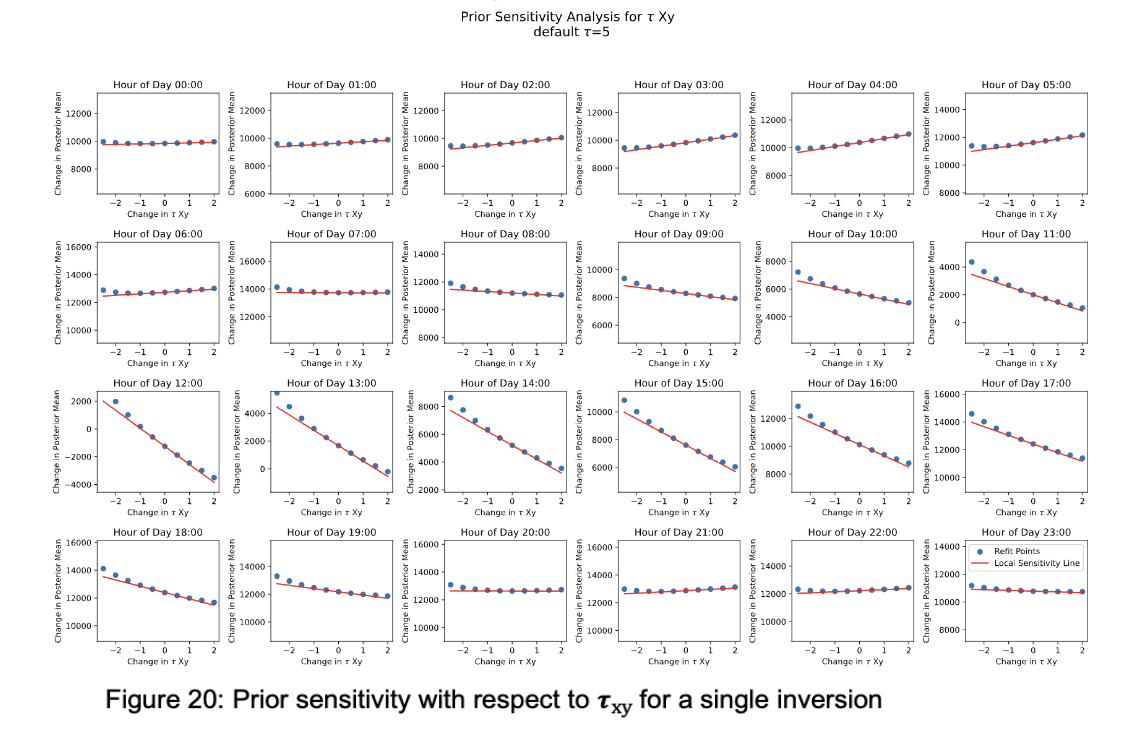
\includegraphics[width=0.8\textwidth]{static_figures/prior.png}
\end{center}

\end{frame}




%%%%%%%%%%%%%%%%%%%%%%%%%%%%%%%%%%%%%
%%%%%%%%%%%%%%%%%%%%%%%%%%%%%%%%%%%%%
%%%%%%%%%%%%%%%%%%%%%%%%%%%%%%%%%%%%%

\begin{frame}[t]{Data influence}

\textbf{Problem: }In inversion problems, the prior is informative, and the model
does smoothing. How is your data being used?  What patterns are possible to
identify?

\textbf{Example question: }Can I detect emissions from road pixels?

\pause
\textbf{Idea: }Let $\r$ be an $N$-vector encoding road pixels.
$$
\r_n = 
\begin{cases}
   1 &\textrm{If observation }n\textrm{ was a road pixel}\\
   0 &\textrm{otherwise}\\
\end{cases}
$$
Suppose we had observed not $\y$, but $\y' = \y + \epsilon \r$.  That is,
$\y'$ is a little more ``roady'' than $\y$.

Then, suppose I used $\y'$ to compute $\x'$.  How much more ``roady'' is $\x'$ than $\x$?

$$
\begin{aligned}
\frac{\textrm{Inferred road pixel change}}{\textrm{Actual road pixel change}} ={}&
\frac{\r^\trans (\x' - \x)}{\r^\trans (\y' - \y)}
\\={}&
\epsilon^{-1} \frac{\r^\trans (\x' - \x)}{\r^\trans \r}
\\={}&
\frac{
\r^\trans
\overbrace{
(\H \B)^\trans \left(
      \H \B \H^\trans + \R
    \right)^{-1}
}^{\textrm{done}}
\r
}{\r^\trans \r}
\end{aligned}
$$

This is just the ``gain matrix'' queried for a particular output.

\textbf{The data influence can be easily estimated from
stuff we already computed.}


\end{frame}


%%%%%%%%%%%%%%%%%%%%%%%%%%%%%%%%%%%%%
%%%%%%%%%%%%%%%%%%%%%%%%%%%%%%%%%%%%%
%%%%%%%%%%%%%%%%%%%%%%%%%%%%%%%%%%%%%

\begin{frame}[c]{Data influence (Tentative preliminary results!)}

\begin{center}
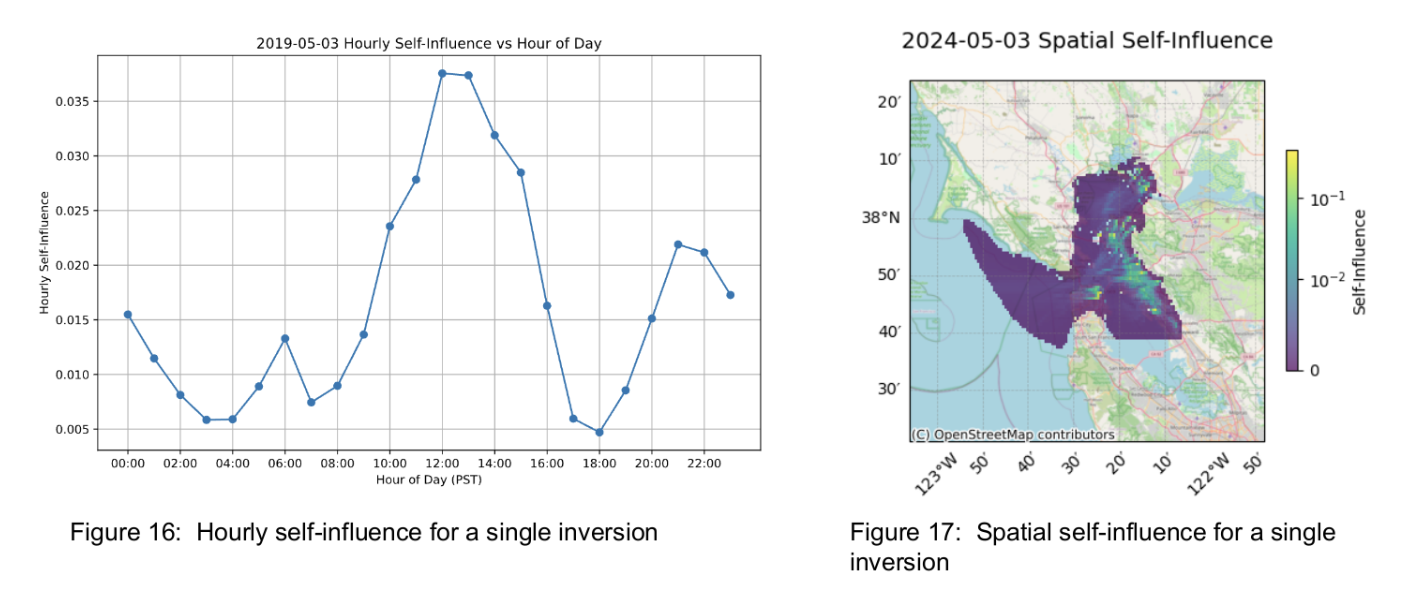
\includegraphics[width=0.8\textwidth]{static_figures/influence.png}
\end{center}


\end{frame}





%%%%%%%%%%%%%%%%%%%%%%%%%%%%%%%%%%%%%
%%%%%%%%%%%%%%%%%%%%%%%%%%%%%%%%%%%%%
%%%%%%%%%%%%%%%%%%%%%%%%%%%%%%%%%%%%%

\begin{frame}[c]{Future work}

   \centering
Lots to do!

\end{frame}








\end{document}
